В истории разные народы использовали системы счисления с разными основаниями. Каждый народ руководствовался своими доводами в пользу того или иного числа в основании. Например, африканские племена использовали 5-ричную систему счисления, потому что на руке 5 пальцев. Тибетцы и нигерийцы использовали 12-ричную, это количество фаланг на четырех пальцах. Привычная нам система счисления с основанием равным 10 появилась в Европе в 16, а в России в 17 веке.
\begin{figure} [h!]
\center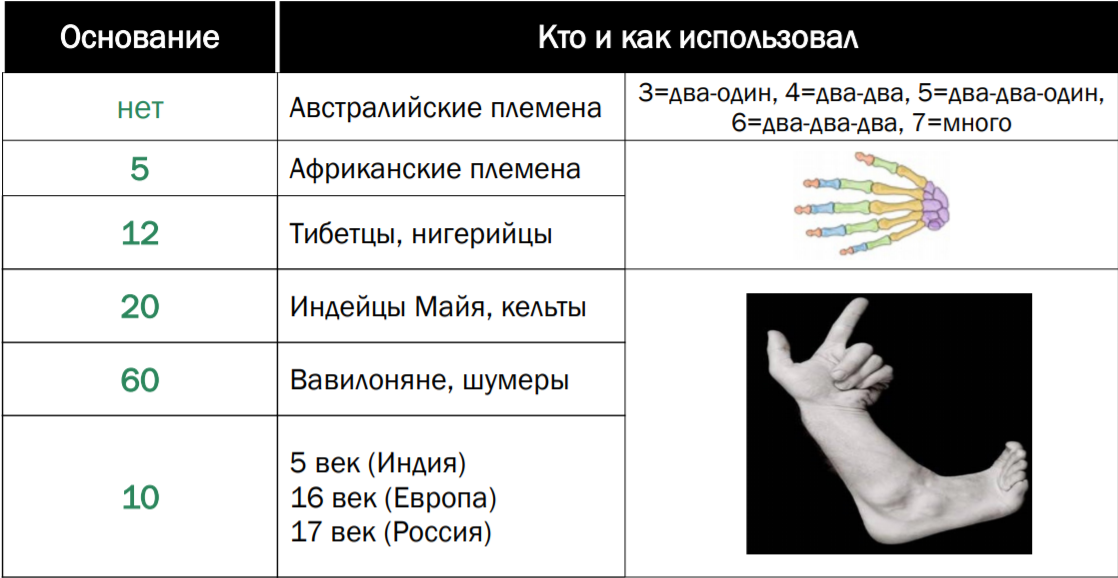
\includegraphics[width=\textwidth]{images/2_1.png}
\caption{Различные системы счисления}
\end{figure}

\section{Позиционная система счисления}

Рассмотрим формулу записи числа в позиционной системе счисления:
\\$X_{(q)} = x_{n-1}\times q^{n-1} + x_{n-2}\times q^{n-2} + ... + x_{1}\times q^{1} + x_{0}\times q^{0} + x_{-1}\hm\times q^{-1}\hm + x_{-2}\hm\times q^{-2}\hm + ... + x_{-m}\times q^{-m}.$
\\Или
\\$$X_{(q)} = \sum_{i=-m}^{n-1} x_{i}\times q^{i},$$
\\где:
\\$X_{(q)}$ - запись числа в системе счисления с основанием $q$;
\\$x_{i}$ - натуральные числа меньше $q$, то есть цифры;
\\$n$ - число разрядов целой части;
\\$m$ - число разрядов дробной части;
\\$q$ - показатель системы счисления.
\\
\\Само число $X_{(q)}$ имеет следующий вид:
\\$$X_{(q)} = x_{n-1}x_{n-2}...x_{1}x_{0}x_{-1}...x_{1-m}x_{-m}.$$
\\Рассмотрим данную формулу на примере:
\\$123,45_{10} = 1\times 10^{2} + 2\times 10^{1} + 3\times 10^{0} + 4\times 10^{-1} + 5\times 10^{-2}$
\\Мы разложили число $123,45$ по этой формуле. В данном случае $q$ = 10, $n$ = 3, $m$ = 2, $X_{(q)} = 123,45$, а $x_{3-1} = 1$ ($x_{2} = 1$), $x_{1} = 2$ и так далее.
\\В позиционной системе счисления важную роль имеет порядок цифр, то есть значение каждого числового знака (цифры) в записи числа зависит от его позиции (разряда).

\section{Перевод чисел из одной системы счисления в другую}

Существуют три способа перевода из одной системы счисления в другую:
\begin{enumerate}
\item Из десятичной системы счисления в систему счисления с основанием $N$.
\item Из системы счисления с основанием $N$ в десятичную систему счисления.
\item Из системы счисления с основанием $N$ в систему счисления с основанием $N^{k}$ и обратно, при условии $k \in \mathbb{N}$.
\end{enumerate}

\subsection{Перевод числа из десятичной системы счисления в систему счисления с основанием $N$}
Чтобы перевести дробное число в систему счисления с основанием $N$ необходимо разделить его на две части: целую и дробную, и каждую часть переводить отдельно.
\subsubsection{Преобразования целой части числа}
Для перевода целой части числа из десятичной системы счисления в другую необходимо:
\begin{enumerate}
\item Разделить целую часть десятичного числа на основание новой системы счисления.
\item Записать остаток деления.
\item Разделить получившийся результат деления (п.1) на основание новой системы счисления (при необходимости).
\item Записать остаток деления.
\end{enumerate}
Повторять, пока целая часть десятичного числа не будет равна 0.
\\Получившиеся в ходе деления остатки и есть цифры искомого числа в новой системе счисления. Записать остатки в обратном порядке (начиная с последнего полученного). Стоит заметить, что в данном способе очень удобно применять деление столбиком.
\\
\\\emph{\textbf{Пример 1:}}
\\\emph{Задание:} перевести число $45_{10}$ в троичную систему счисления.
\\\emph{Решение:} последовательно разделим $45_{10}$ на $3$, записывая остатки:
\begin{figure}[h]
\centering
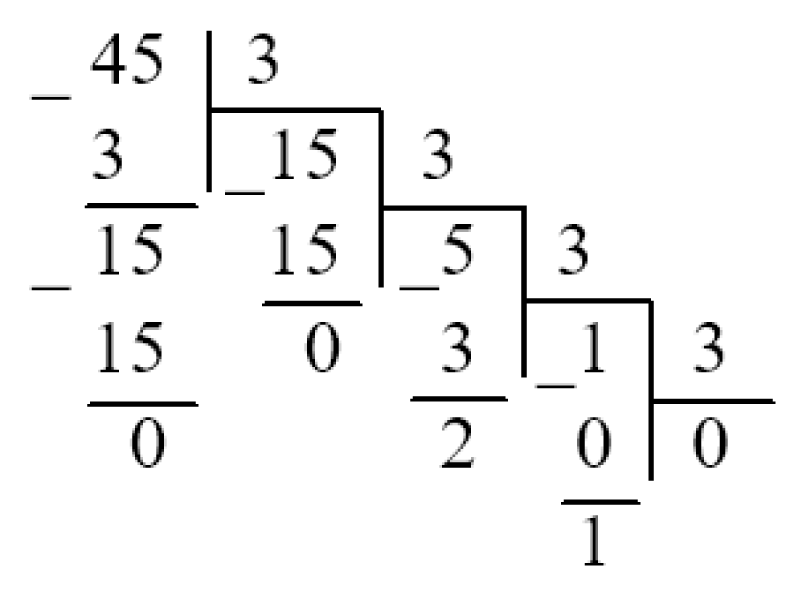
\includegraphics[width=4cm]{1_2_1(1)}
\caption{Последовательное деление $45_{10}$ на $3$.}
\end{figure}
\\Полученные остатки: 0, 0, 2, 1. Записываем их в обратном порядке.
\\Ответ:$45_{10} = 1200_{3}$

\subsubsection{Преобразования дробной части числа}
Для перевода дробной части числа из десятичной системы счисления в другую необходимо:
\begin{enumerate}
\item Умножить дробную часть десятичного числа на основание новой системы счисления.
\item Отделить и записать целую часть.
\item Умножить дробную часть результата умножения (п.1) на основание новой системы счисления (при необходимости).
\item Отделить и записать целую часть.
\end{enumerate}
Повторять, пока дробная часть десятичного числа не будет равна 0.
\\Получившиеся в ходе умножения целые части и есть цифры искомого числа в новой системе счисления. Записать целые части в прямом порядке (начиная с первого полученного). Первая записанная целая часть (0) идет в целую часть нового числа, а в дробную записываются полученные целые части, начиная со второй. Стоит заметить, что в данном способе очень удобно применять умножение столбиком.
\\
\\\emph{\textbf{Пример 2:}}
\\\emph{Задание:} перевести число $0,625_{10}$ в четверичную систему счисления.
\\\emph{Решение:} умножим дробную часть $0,625_{10}$ на $4$, записывая целые части, пока не получим в дробной части 0:
\begin{figure}[h]
\centering
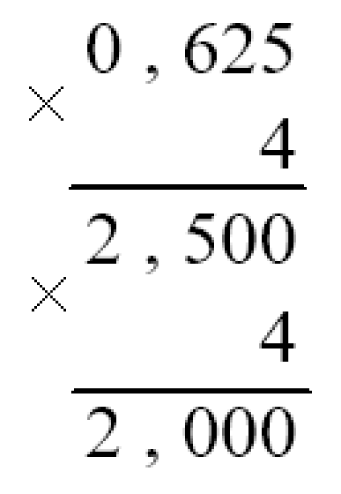
\includegraphics[width=1.7cm]{1_2_1(2)}
\caption{Умножение $0,625_{10}$ на $4$ до получения 0 в дробной части.}
\end{figure}
\\\emph{Пояснение: сначала умножаем 0,625 на 4, получаем 2,5. 2 записываем в целые части, а далее используем дробную часть -- 0,5. Умножаем 0,5 на 4, получаем 2, записываем в целые части. Так как дробная часть равна 0, то перевод окончен.}
\\Полученные целые части: 0, 2, 2. Первая полученная целая часть (0) идет в целую часть нового числа. Остальные (2, 2) в дробную часть.
\\Ответ: $0,625_{10} = 0,22_{4}$.
\\
\\\emph{\textbf{Пример 3:}}
\\\emph{Задание:} перевести число $43,52_{10}$ в пятеричную систему счисления.
\\\emph{Решение:} разделим $43,52_{10}$ на две части: целую ($43_{10}$) и дробную ($0,52_{10}$). Переведем целую и дробную части по отдельности:
\begin{figure}[h]
\centering
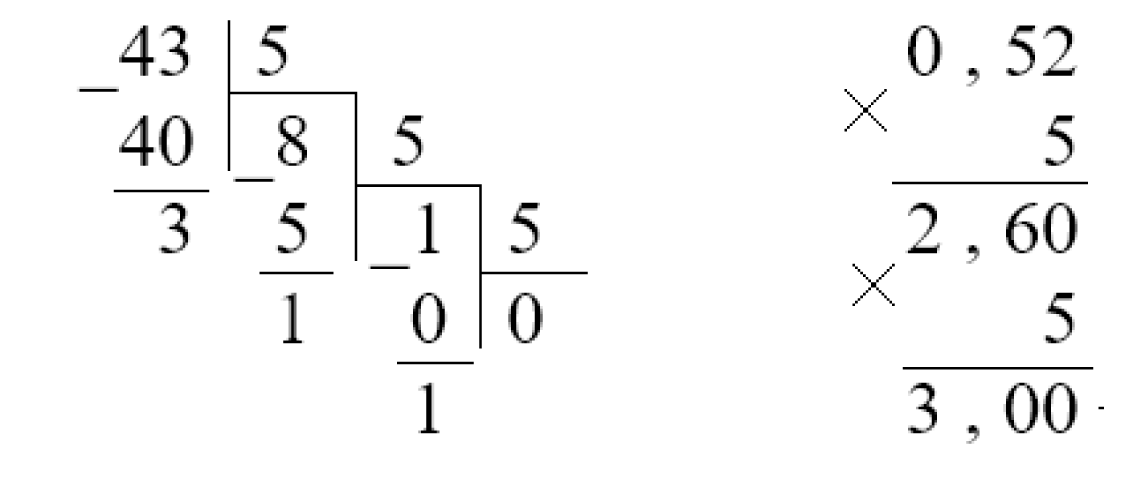
\includegraphics[width=6cm]{1_2_1(3)}
\caption{Перевод целой и дробной частей.}
\end{figure}
\\Полученные остатки (3, 1, 1) запишем в обратном порядке: $43_{10} = 113_{5}$
\\Полученные целые части (0, 2, 3) запишем в прямом порядке: $0,52_{10} = 0,23_{5}$
\\Объеденим полученные части
\\Ответ: $43,52_{10} = 113,23_{5}$.

\subsection{Перевод числа из системы счисления с основанием $N$ в десятичную систему счисления}
Формула перевода числа из системы счисления с основанием $N$ в десятичную систему счисления это практически формула записи числа в позиционной системе счисления.
$$X_{(10)} = \sum_{i=-m}^{n-1} x_{i}\times q^{i},$$
\\где:
\\$X_{(10)}$ - искомое число в десятичной системе счисления
\\$x_{i}$ - натуральные числа меньше $q$, то есть цифры
\\$n$ - число разрядов целой части
\\$m$ - число разрядов дробной части
\\$q$ - показатель системы счисления
\\
\\\emph{\textbf{Пример 1:}}
\\\emph{Задание:} перевести число $1101,111_{2}$ в десятичную систему счисления.
\\\emph{Решение:} $1101,111_{2} = 1\times 2^{3} + 1\times 2^{2} + 0\times 2^{1} + 1\times 2^{0} + 1\times 2^{-1} + 1\hm\times 2^{-2}\hm + 1\hm\times 2^{-3}\hm = 1\times 8 + 1\times 4 + 0\times 2 + 1\times 1 + 1\times 0,5 + 1\times 0,25 + 1\times 0,125\hm = 8 + 4 + 1 + 0,5 + 0,25 + 0,125 = 13,875_{10} $
\\Ответ: $1101,111_{2} = 13,875_{10}.$

\subsection{Перевод числа из системы счисления с основанием $N$ в систему счисления с основанием $N^{k}$ и обратно, при условии $k \in \mathbb{N}$}

Если основание системы счисления первого числа является степенью основания системы счисления второго числа ($N = N^{k}$), при условии $k \in \mathbb{N}$, то можно использовать следующий алгоритм.
\begin{center}
\center{\textbf{Преобразование $N \to N^{k}$}}
\end{center}

\begin{enumerate}
\item Дополнить число (записанное в системе счисления $N$) незначащими нулями так, чтобы количество цифр было кратно $k$ (если число дробное, то дополнить так, чтобы и в целой и в дробной частях количество цифр было кратно $k$).
\item Разбить это число на группы по $k$ цифр, начиная от нуля (если число дробное, то целую часть разбивать, начиная от запятой в левую сторону, а дробную часть, начиная от запятой в правую сторону).
\item Заменить каждую такую группу эквивалентным числом, записанным в системе $N^{k}$.
\end{enumerate}

\begin{center}
\center{\textbf{Преобразование $N^{k} \to N$}}
\end{center}
\begin{table}[h!]
\caption{Основания вида $2^{k}$}
\centering
\begin{tabular}{|c|c|c|c|c|}
\hline
10--ая & 2--ая & 4--ая & 8--ая & 16--ая
\\\hline
0 & 0000 & 000 & 00 & 0
\\ 1 & 0001& 001 & 01 & 1
\\ 2 & 0010 & 002 & 02 & 2
\\ 3 & 0011 &003 & 03 & 3
\\ 4 & 0100 & 010 & 04 & 4
\\ 5 & 0101 & 011 & 05 & 5
\\ 6 & 0110 & 012 & 06 & 6
\\ 7 & 0111 & 013 & 07 & 7
\\ 8 & 1000 & 020 & 10 & 8
\\ 9 & 1001 & 021 & 11 & 9
\\ 10 & 1010 & 022 & 12 & A
\\ 11 & 1011 & 023 & 13 & B
\\ 12 & 1100 & 030 & 14 & C
\\ 13 & 1101 & 031 & 15 & D
\\ 14 & 1110 & 032 & 16 & E
\\ 15 & 1111 &300 & 17 & F
\\\hline
\end{tabular}
\end{table}

\begin{enumerate}
\item Заменить каждую цифру числа, записанного в системе счисления $N^{k}$, эквивалентным набором из $k$ цифр системы счисления $N$.
\end{enumerate}

Рассмотрим данный метод на системах счисления с основанием $N = 2^{k}$. Для этого воспользуемся таблицей 2.1.\\


\emph{\textbf{Пример 1:}}
\\\emph{Задание:} пользуясь таблицей перевести число $1542,43_{8}$ в двоичную систему счисления
\\\emph{Решение:} по таблице находим чему равны цифры исходного числа в двоичной системе. $1_{8} = 001_{2}$, $5_{8} = 101_{2}$ (незначащие нули убираем, так как необходимо, чтобы количество цифр в эквивалентном наборе было равно степени $k$ из выражения $N = N^{k}$, где $N^{k}$ - исходная система счисления. В данном случае $k = 3$) и так далее.
\\Заменяем каждую цифру числа эквивалентным набором.
\\Ответ: $1542,43_{8} = 001101100010,100011_{2}$
\\

\emph{\textbf{Пример 2:}}
\\\emph{Задание:} пользуясь таблицей перевести число $11010,11_{2}$ в шестнадцатиричную систему счисления
\\\emph{Решение:} первым делом, добавим незначащие нули так, чтобы количество цифр было кратно $k$ (в данном случае $k = 4$). Так как число дробное, не забываем добавлять нули и в конце числа. \\Получим $00011010,1100_{2}$.
\\Теперь необходимо разбить число на группы по $k$ цифр (начинаем от запятой). Результат: $0001\ 1010\ ,\ 1100\ _{2}$.
\\Пользуясь таблицей, заменяем группы цифр эквивалентными числами, записанным в шестнадцатиричной системе счисления.
\\Ответ: $11010,11_{2} = 1A,C_{16}$.


\section{Оптимальная система счисления}
Давайте представим, что Вы по несчастливой (или счастливой) случайности попали на необитаемый остров. Обеспокоенный количеством дней, которые Вам суждено провести на острове в ожидании спасателей, Вы решаете вести счет дней с помощью камней. Но вот незадача - камней на острове нашлось всего 60 штук (небогатый на камни остров оказался). И для того, чтобы вести учет дней как можно продуктивнее (учесть как можно больше дней) необходимо выбрать систему счисления, плотность записи числа которой максимальна при данных обстоятельствах.
\\Существует зависимость плотности записи информации от основания системы счисления. Если взять $N$ камней, а за основание принять число $X$, то получится $^N/_X$ разрядов, которыми можно закодировать $X^{^N/_X}$ чисел.
\\То есть с помощью 60 камней мы можем закодировать: $2^{30}$, $3^{20}$, $4^{15}$, $5^{12}$, $6^{10}$, $10^{6}$, $12^{2}$, $15^{4}$, $20^{3}$, $30^{2}$ или $60^1$ чисел. Все зависит от того, какую систему счисления мы выберем. Возведя все числа в степени, мы увидим, что самое большое из них это $3^{20} = 3486784401$.
\\Удельная натуральнологарифмическая плотность записи числа зависит от основания системы счисления $х$ и выражается функцией $y = \frac{\ln{x}}{x}$. Эта функция имеет максимум при $x = e = 2,718281828...$.\\
\\\emph{Рассмотрим следующую задачу:} Робинзон Крузо нашёл на острове 60 камней. Сколько прошедших дней можно ими закодировать в разных системах счисления?
\begin{figure}[h]
\centering

\includegraphics[width=12cm]{images/1_2_3(10CC)}
\caption{Пример кодирования номера дня}
\end{figure}
\\Возможные варианты в других системах счисления:
$2^{30}, 3^{20}, 4^{15}, 5^{12}, 6^{10}, 7^{8},\\ 8^7, 9^6, 10^6, 11^5, 12^5, ..., 20^3, ..., 30^2, ..., 60^1$
\\\\В какой системе счисления количество кодируемых дней наибольшее?
\\\\Если взять N камней, а за основание CC принять число X, то получится $N/X$ разрядов,которыми можно закодировать $y=X^{N/X}$ дней (для простоты полагаем, что количество разрядов может быть нецелым).
\begin{figure}[h]
\centering
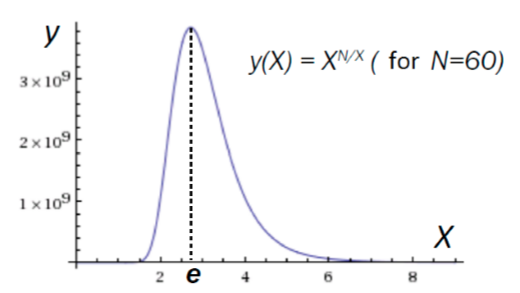
\includegraphics[width=8cm]{1_2_3(1)}
\caption{Основание оптимальной системы счисления}
\end{figure}
\\Таким образом, самая оптимальная система счисления имеет основание равное $e = 2,718281828...$, то есть нецелочисленное. Она обладает наибольшей плотностью записи информации.
\\Возвращаясь к нашему пребыванию на острове, мы не можем взять дробное основание для системы счисления. Поэтому мы берем самое близкое целое к $e$ - это $3$.

\section{Округление чисел}

Как происходит округление чисел в десятичной системе счисления? Каждый учил в школе правила округления: 1, 2, 3, 4 округляется в меньшую сторону, а 5, 6, 7, 8 и 9 - в большую.
Рассмотрим два примера:
\\
\\
\begin{minipage}[c]{6cm}
\begin{center}
\begin{tabular}{|c|c|c|}
\hline  & Число & Округление
\\\hhline{~--} & 5,9 & 6,0
\\ & 4,1 & 4,0
\\ & 5,0 & 5,0
\\ & 6,6 & 7,0
\\ & 2,4 & 2,0
\\\hline Cумма & 24,0 & 24,0
\\\hline
\end{tabular}
\emph{Пример 1}
\newline
\end{center}
\end{minipage}
\begin{minipage}[c]{6cm}
\begin{center}
\begin{tabular}{|c|c|c|}
\hline & Число & Округление
\\\hhline{~--}  & 5,5 & 6,0
\\ & 3,5 & 4,0
\\ & 2,5 & 3,0
\\ & 8,5 & 9,0
\\ & 1,5 & 2,0
\\\hline Cумма & 21,5 & 24,0
\\\hline
\end{tabular}
\emph{Пример 2}
\newline
\end{center}
\end{minipage}


В примере 1 мы видим, что сумма до и после округления одинакова. Так случилось, потому что мы округляли то в большую сторону, то в меньшую, и в итоге количество округлений в большую сторону равно количеству округлений в меньшую. Округление нам не помешало получить красивую сумму.
\\А теперь посмотрим на специально подобранный пример 2. Разница сумм довольно большая. Так получилось, потому что мы округляли всегда только в большую сторону, хотя мы округляли по правилам.
\\Если проделать такой эксперимент с большим количеством чисел (тысяча, две тысячи или даже больше), то ошибка будет небольшая, но она будет.
\\Работая с числами, у которых показатель системы счисления четный, мы натыкаемся на следующую проблему: у нас нечетное количество чисел для округления. Разберем на примере десятичной системы счисления. В ней всего 10 цифр - 0, 1, 2, 3, 4, 5, 6, 7, 8, 9. Числа $X.0$ мы не округляем. Остается 9 чисел: $X.1$, $X.2$, $X.3$, $X.4$ округляем в меньшую сторону (всего 4 числа), а $X.5$, $X.6$, $X.7$, $X.8$, $X.9$ - в большую (всего 5 чисел). $X.5$ - середина между $X+1$ и $X$, однако мы округляем в пользу $X+1$, то есть в большую. Таким образом, при работе с большим количеством чисел, мы всегда будем округлять в большую сторону чаще, чем в меньшую. Отсюда и ошибка в итоговой сумме.
\\Чтобы этого избежать, некоторые программы при автоматическом округлении большого количества чисел округляют $X.5$ по очереди то в большую сторону, то в меньшую.
\\В системах счисления с нечетным основанием такой ошибки нет. Возьмем, к примеру, пятиричную систему счисления. Она содержит цифры 0, 1, 2, 3, 4. Числа $X.0$ мы не округляем, остается 4 числа: $X.1$, $X.2$ округляем в меньшую сторону (всего 2 числа), а $X.3$, $X.4$ - в большую (всего 2 числа). Таким образом, количество чисел, округленных в меньшую сторону, равно количеству чисел, округленных в большую.
\textbf{Варианты решения задачи накопления ошибок округления:}
\begin{enumerate}
\item \emph{Случайное округление:} датчик случайных чисел используется при принятии решений о том, следует ли округлять число вверх или вниз
\item \emph{Банковское округление(до ближайшего четного):} $3.5 \approx 4$, но $2.5 \approx 2$
\item \emph{До ближайшего нечетного:} $3.5 \approx 3$, но $2.5 \approx 3$. \\Анологично $4.3_{(6)} \approx 5_{(6)} $
\item \emph{Чередующееся:} направление округления меняется на противоположное при
каждой операции округления (необходимо «помнить» о предыдущем округлении).
\end{enumerate}
\textbf{Примечание:} Каждое из правил можно применять как полностью
универсально, так и комбинировано с классическим правилом округления,
дополняя его лишь при округлении пограничных значений.
\section{Нетрадиционные системы счисления}
\subsection{Факториальная система счисления}
Любое натуральное число можно представить в виде $$ X = \sum^{n}_{k = 1} d_{k}\times k! \qquad \mbox{,где  } 0 \leqslant d_{k} \leqslant k $$
\\В основании факториальной системы счисления используется факториал.
\\Запись числа в факториальной системе счисления будет иметь вид $$X_{\mbox{ф}} = d_{n}d_{n-1}...d_{1}.$$

\subsubsection{Перевод из факториальной системы счисления в десятичную}
Алгоритм перевода из факториальной системы счисления в десятичную очень похож на алгоритм перевода из системы счисления с основанием $N$ в десятичную (раздел 2.2.1).
$$ X_{10} = d_{n}\times n! + d_{n-1}\times (n-1)! + d_{n-2}\hm\times (n-2)!\hm + ...\hm + d_{2}\times 2! + d_{1}\times 1!,$$
где:
\\$X_{10}$ - искомое число в десятичной системе счисления;
\\$d_{i}$ - натуральные числа меньше или равные $i$;
\\$n$ - количество разрядов исходного числа.
\\
\emph{\textbf{Пример 1:}}
\\\emph{Задание:} перевести число $221_{\mbox{ф}}$ в десятичную систему счисления.
\\\emph{Решение:} $221_{\mbox{ф}} = 2\times 3! + 2\times 2! + 1\times 1! = 2\times 6 + 2\times 2 + 1\times 1 = 12 + 4 + 1 = 17_{10}$
\\Ответ:  $221_{\mbox{ф}} = 17_{10}$.
\subsubsection{Перевод из десятичной системы счисления в факториальную}
Для перевода воспользуемся все той же формулой:
$$ X_{10} = d_{n}\times n! + d_{n-1}\times (n-1)! + d_{n-2}\hm\times (n-2)!\hm + ...\hm + d_{2}\times 2! + d_{1}\times 1!$$
Стоит обратить внимание, что $0 \leqslant d_{1}\leqslant 1$; $0 \leqslant d_{2}\leqslant 2$ и так далее.
\begin{enumerate}
\item Находим факториал $k!$, значение которого больше $X_{10}$, но ближе всего к нему. Тогда $n = k - 1$, где $n$ - количество разрядов искомого числа в факториальной системе.
\item Записываем $$ X_{10} = d_{n}\times n! + d_{n-1}\times (n-1)! + d_{n-2}\hm\times (n-2)!\hm + ...\hm + d_{2}\times 2! + d_{1}\times 1!$$ с уже полученным $n$.
\item Начиная с $d_{n}$ с помощью ума и смекалки начинаем подбирать коэффициенты, помня, что $d_{1} \in \{0,1\}$, $d_{2} \in \{0,1,2\}$ и т.д.
\end{enumerate}

\emph{\textbf{Пример 2:}}
\\\emph{Задание:} перевести число $54_{10}$ в факториальную систему счисления.
\\\emph{Решение:} $54_{10} < 5! (5! = 120)$, значит количество разрядов равно $5 - 1 = 4$.
\\Запишем формулу для $n = 4$: $54_{10} = d_{4}\times 4! + d_{3}\times 3! + d_{2}\times 2!\hm + d_{1}\hm\times 1!$
\\Подберем коэффициенты: $54_{10} = 2\times 4! + 1\times 3! + 0\times 2!\hm + 0\hm\times 1!$
\\Ответ:  $54_{10} = 2100_{\mbox{ф}}$.
\\
\\\textbf{Применение факториальной системы счисления:} декодирование и кодирование перестановок.
\\\\Перестановками называют комбинации, состоящие из одних и тех же $n$ различных элементов и отличающиеся только порядком их расположения. \\\\Число возможных перестановок рассчитывается по формуле:
\\$P_n=n!$
$n! = 1*2*3…*n,$ причем $0! = 1, 1! = 1$\\
Важно отметить, что первая перестановка имеет номер 0.\\\\

\begin{minipage}[c]{9cm}
\emph{\textbf{Пример 3:}}
\\\emph{Задание:} Имеется $n = 5$ чисел (1, 2, 3, 4, 5), нужно найти все их перестановки. Известно, что существует $n! = 5! = 120$ таких перестановок. Найти перестановку, если известен ее номер $k = 52$.
\\\emph{Решение:} Переведем $k$ в факториальную систему: $52_{10} = 2\times 4! + 0\times 3! + 2\times 2!\hm + 0\hm\times 1! = 2020_{\mbox{ф}}$.
\\Дополним результат до $n - 1$ разрядов (при необходимости), расставим символы по местам:
%\begin{enumerate}
\\1. Справа от $5$ есть $2$ меньшие цифры\ $(- - 5 - -)$.
\\2. Справа от $4$ есть $0$ меньших цифр\ \ \ $(- - 5\ - 4)$.
\\3. Справа от $3$ есть $2$ меньшие цифры\ $(3\ - 5\ - 4)$.
\\4. Справа от $2$ есть $0$ меньших цифр\ \ \ $(3\ - 5\ \ 2\ \ 4)$.
\\Ответ: (3\ 1\ 5\ 2\ 4).
%\end{enumerate}
\end{minipage}
\begin{minipage}[c]{2.5cm}
\begin{tabular}{|c|c|}
\hline  0 & 12345
\\ 1 & ?????
\\ ... & .....
\\ 52 & ?????
\\ ... & .....
\\ 119 & 54321
\\\hline
\end{tabular}
\end{minipage}
\subsection{Система счисления Цекендорфа}
Любое натуральное число можно представить в виде
$$ X = \sum^{n}_{k = 1} d_{k}\times F_{k}, \qquad \mbox{ где  } d_{k} \in \{0,1\},\mbox{а } F_{k} \mbox{ - числа Фибоначчи}. $$
Каждое число Фибоначчи есть сумма двух предыдущих чисел:
\\ $F_{k} = \{1, 1, 2, 3, 5, 8, 13, 21, ...\}$.
\\В записи чисел в системе счисления Цекендорфа первая единица из ряда чисел Фибоначчи \textbf{не используется}(т.к. первая единица это $F_{0}$).
\\Запись числа в системе счисления Цекендорфа будет иметь вид $$X_{\mbox{ц}} = d_{n}d_{n-1}...d_{1}.$$
В записи чисел в системе счисления Цекендорфа \textbf{не допускается использование двух единиц подряд}.
\subsubsection{Перевод из системы счисления Цекендорфа в десятичную}
Алгоритм перевода из системы счисления Цекендорфа в десятичную очень похож на алгоритм перевода из системы счисления с основанием $N$ в десятичную (раздел 2.2.1).
$$ X_{10} = d_{n}\times F_{n} + d_{n-1}\times F_{n-1} + d_{n-2}\hm\times F_{n-2}\hm + ...\hm + d_{2}\times F_{2} + d_{1}\times F_{1},$$
где:
\\$X_{10}$ - искомое число в десятичной системе счисления;
\\$d_{i}$ - число, принимающее значение 0 или 1;
\\$n$ - количество разрядов исходного числа.
\\
\\\emph{\textbf{Пример 1:}}
\\\emph{Задание:} перевести число $100101_{\mbox{ц}}$ в десятичную систему счисления.
\\\emph{Решение:} $100101_{\mbox{ц}} = 1\times 13 + 0\times 8 + 0\times 5 + 1\times 3 + 0\times 2 + 1\times 1 = 13 + 3 + 1 = 17_{10}$.
\\Ответ:  $100101_{\mbox{ц}} = 17_{10}$.
\subsubsection{Перевод из десятичной системы счисления в систему счисления Цекендорфа}
Для перевода воспользуемся все той же формулой:
$$ X_{10} = d_{n}\times F_{n} + d_{n-1}\times F_{n-1} + d_{n-2}\hm\times F_{n-2}\hm + ...\hm + d_{2}\times F_{2} + d_{1}\times F_{1}.$$

\begin{enumerate}
\item Находим число $F_{k}$ в ряду чисел Фибоначчи, которое больше $X_{10}$, но ближе всего к нему. Тогда $n = k - 1$, где $n$ - количество разрядов искомого числа в системе Цекендорфа;
\item Записываем $$ X_{10} = d_{n}\times F_{n} + d_{n-1}\times F_{n-1} + d_{n-2}\hm\times F_{n-2}\hm + ...\hm + d_{2}\times F_{2} + d_{1}\hm\times F_{1}.$$ с уже полученным $n$;
\item Начиная с $d_{n}$ с помощью ума и смекалки начинаем подбирать коэффициенты, помня, что $d_{1} \in \{0,1\}$, и что две единицы не могут стоять рядом.
\end{enumerate}

\emph{\textbf{Пример 2:}}
\\\emph{Задание:} перевести число $19_{10}$ в систему счисления Цекендорфа.
\\\emph{Решение:} $19_{10} < 21 (21 = F_{7})$, значит количество разрядов равно $7 - 1 = 6$.
\\Запишем формулу для $n = 6$: $d_{6}\times 13 + d_{5}\times 8 + d_{4}\hm\times 5 + d_{3}\hm\times 3 + d_{2}\hm\times 2\hm + d_{1}\hm\times 1$
\\Подберем коэффициенты: $19_{10} = 1\times 13 + 0\times 8 + 1\hm\times 5 + 0\hm\times 3 + 0\hm\times 2\hm + 1\hm\times 1$
\\Ответ:  $19_{10} = 101001_{\mbox{ц}}$.
\\
\\\textbf{Применение системы счисления Цекендорфа:} кодирование данных с маркером завершения $ \textquotesingle 11\textquotesingle $ , у некоторых народов в сельском хозяйстве - минимизация необходимого числа зерен.

\subsection{Система счисления Бергмана}
Любое действительное неотрицательное число можно представить в виде:
$$ X = \sum^{\infty}_{k = -\infty} d_{k}\times z^{k} \qquad \mbox{,где  } d_{k} \in \{0,1\},\mbox{а } z = \frac{1+\sqrt{5}}{2}.$$
Число $z$ - число золотой пропорции.
\\Запись числа в системе счисления Бергмана будет иметь вид: $$X_{\mbox{Б}} = d_{n}d_{n-1}...d_{2}d_{1}d_{0},d_{-1}d_{-2}...d_{-m}.$$
Чтобы исключить неоднозначность, используется запись с наибольшим количеством разрядов.
\subsubsection{Перевод из системы счисления Бергмана в десятичную}
Алгоритм перевода из системы счисления Бергмана в десятичную очень похож на алгоритм перевода из системы счисления с основанием $N$ в десятичную (раздел 2.2.1).
$$ X_{10} = d_{n}\times z^{n} + d_{n-1}\times z^{n-1} + ...\hm + d_{2}\times z^{2} + d_{1}\hm\times z^{1}\hm + d_{0}\times z^{0}\hm + d_{-1}\times z^{-1}\ + ... d_{-m}\times z^{-m},$$
где:
\\$X_{10}$ - искомое число в десятичной системе счисления;
\\$d_{i}$ - число, принимающее значение 0 или 1;
\\$n$ - количество разрядов целой части;
\\$m$ - количество разрядов дробной части.
\\
\\\emph{\textbf{Пример 1:}}
\\\emph{Задание:} перевести число $100,01_{\mbox{Б}}$ в десятичную систему счисления.
\\\emph{Решение:} $100,01_{\mbox{Б}} = 1\times (\frac{1+\sqrt{5}}{2})^{2} + 0\times (\frac{1+\sqrt{5}}{2})^{1} + 0\times (\frac{1+\sqrt{5}}{2})^{0} + 0\times (\frac{1+\sqrt{5}}{2})^{-1}\hm + 1\hm\times (\frac{1+\sqrt{5}}{2})^{-2} = (\frac{1+\sqrt{5}}{2})^{2} + (\frac{1+\sqrt{5}}{2})^{-2} = \frac{6+2\sqrt{5}}{4} + \frac{4}{6+2\sqrt{5}} = \frac{9 + 3\sqrt{5}}{3+\sqrt{5}} = \frac{3(3 + \sqrt{5})}{3+\sqrt{5}} = 3.$
\\Ответ:  $100,01_{\mbox{Б}} = 3_{10}.$
\\{\small\textbf{Перевод чисел из десятичной системы в систему счисления Бергмана происходит методом подбора}}
\\\\
\textbf{Применение системы счисления Бергмана:}  запись иррациональных чисел конечным числом цифр, контроль арифметических операций, коррекция ошибок, самосинхронизация кодовых последовательностей при передаче по каналу связи.

\subsection{Нега-позиционная система счисления}
Это системы счисления с отрицательным основанием. Числа в нега-позиционных системах счисления, которые содержат четное количество цифр -- отрицательные.
\\Главная особенность таких систем в том, что не нужно никаких специальных знаков для обозначения отрицательных чисел.
\\
\\\textbf{Перевод чисел из нега-позиционных систем счисления полностью описан в разделе 2.2.1. Обратный перевод происходит методом подбора.}
\\
\\\emph{Примеры в нега-десятичной системе счисления:}
\\$15_{-10} = 1\times (-10)^1 + 5\times (-10)^0 = - 1\times 10 + 5\times 1 = -10 + 5 = -5_{10}$;
\\$582_{-10} = 5\times (-10)^2 + 8\times (-10)^1 + 2\times (-10)^0 = 5\times 100 - 8\times 10 + 2\times 1\hm = 500 - 80 + 2 = 422_{10}$.
\subsection{Симметричная система счисления}
Это системы счисления с отрицательными числами. Центром симметрии является 0, поэтому основанием для таких систем счисления могут быть только нечетные числа.
\\Главная особенность таких систем, как и нега-позиционных, в том, что не нужно никаких специальных знаков для обозначения отрицательных чисел.
\\
\\\textbf{Перевод чисел из симметричных систем счисления и полностью описан в разделе 2.2.1. Обратный перевод происходит методом подбора.}
\\
\\\emph{Примеры в симметричной пятеричной системе счисления:}
Если в обычной пятеричной системе используются цифры \{0, 1, 2, 3, 4\}, то в симметричной пятеричной системе используются \{-2, -1, 0, 1, 2\}.
\\$10\overline{2}\overline{1}2_{5\mbox{С}} = 1\times 5^4 + 0\times 5^3 + (-2)\times 5^2 + (-1)\times 5^1 + 2\hm\times 5^0\hm = 1\times 625 + 0\times 125 - 2\times 25 - 1\times 5 + 2\hm\times 1\hm= 625 - 50 - 5 + 2 = 572_{10}$;
\\$\overline{1}021\overline{2}_{5\mbox{С}} = (-1)\times 5^4 + 0\times 5^3 + 2\times 5^2 + 1\times 5^1 + (-2)\hm\times 5^0\hm = - 1\times 625 + 0\times 125 + 2\times 25 + 1\times 5 - 2\hm\times 1\hm= - 625 + 50 + 5 - 2 = -572_{10}$.

Стоит обратить внимание, что цифры с чертой сверху - отрицательные.